\part{Theoretical Background}

\chapter{Precision Agriculture and Smart Irrigation}

\section{Introduction}

Precision agriculture is a management approach that uses data and technology to adapt agricultural practices to spatial and temporal variability. Instead of treating a field as a uniform entity, precision agriculture recognizes that soil properties, water availability, crop development, microclimate, pest pressure, and nutrient status can differ across zones and over time. This approach is especially important for irrigation, where uniform schedules may over-irrigate some areas and under-irrigate others.

Smart irrigation is the application of sensing, communication, computation, and control to irrigation management. It aims to apply water according to actual crop and soil needs. In the literature, smart irrigation systems are often described as combinations of sensors, wireless networks, cloud platforms, control units, data processing, and user interfaces. García et al. [7] review sensors, nodes, wireless technologies, and irrigation actuators used in IoT-based irrigation systems, while Obaideen et al. [8] emphasize the role of soil and weather monitoring in achieving water-use efficiency.

In this thesis, smart irrigation is understood as an operational system that can measure relevant variables, transmit them to a processing layer, infer the irrigation need, and support or execute irrigation decisions. The proposed Agrio platform follows this definition but extends it through a Digital Twin layer that keeps a virtual state of the irrigation zone and simulates future moisture evolution.

\begin{figure}[H]
    \centering
    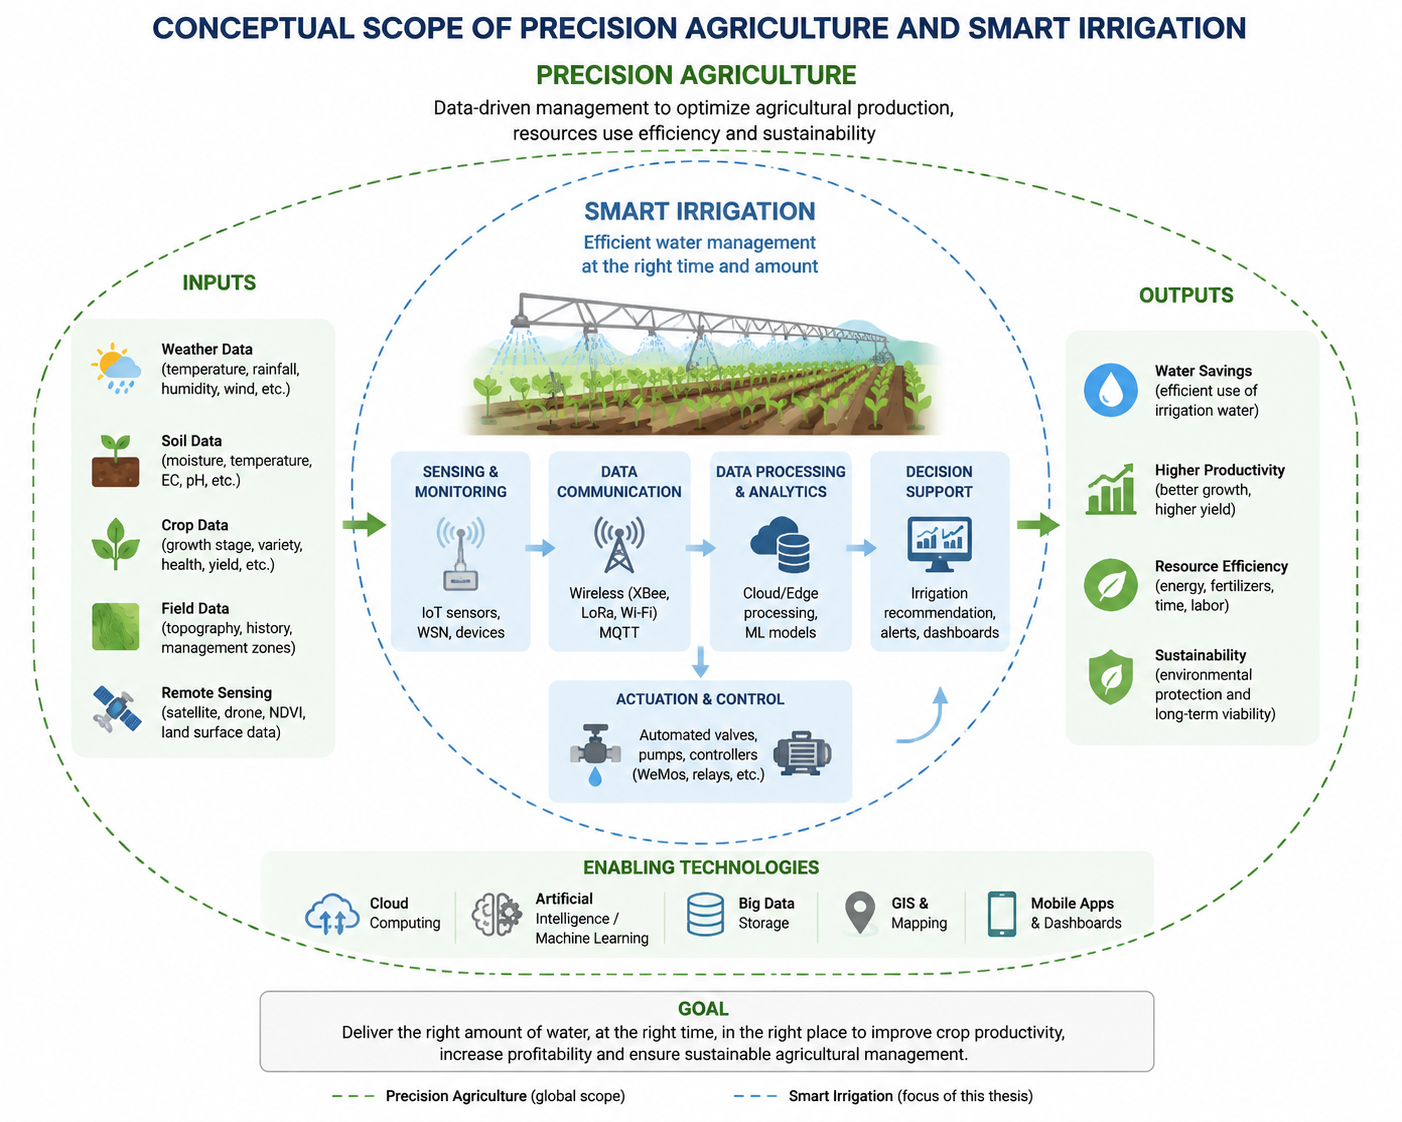
\includegraphics[width=0.9\textwidth]{figures/chapter_01/Figure 1.1 — Conceptual scope of precision agriculture and smart irrigation.png}
    \caption{Conceptual scope of precision agriculture and smart irrigation. Source: Authors.}
    \label{fig:1-1-conceptual-scope-of-precision-agriculture-and-smart-irrigation}
\end{figure}

\section{Water scarcity and irrigation management}

Water scarcity is one of the main motivations behind intelligent irrigation research. Several reviewed papers remind that agriculture accounts for a large share of global freshwater withdrawals, often around 70\%. This fact is used in many irrigation and Digital Twin studies to justify the need for more efficient water management. The issue is not only environmental; it is also economic and social. Water scarcity can reduce yields, increase food prices, and make agricultural production more vulnerable to drought and climate variability.

Irrigation scheduling is the process of deciding when and how much water should be applied. Classical scheduling may rely on fixed calendars, farmer experience, empirical observation of soil moisture, crop coefficients, or soil water balance methods. These methods can be effective when they are correctly calibrated, but they may become inaccurate when weather, soil, crop stage, or irrigation infrastructure changes. In real agricultural environments, local conditions can cause deviations between estimated and actual crop water consumption.

In the context of this project, the water management problem is addressed at prototype scale. The objective is not to claim immediate large-scale water saving, but to design and validate a technical architecture capable of supporting precise irrigation decisions. This distinction is important academically: the prototype proves the feasibility of the Digital Twin workflow, while future field trials are required to quantify agronomic and economic water savings under real farm conditions.

\section{From conventional irrigation to smart irrigation}

Conventional irrigation methods include flood irrigation, furrow irrigation, sprinkler irrigation, drip irrigation, and manual watering. Each method has advantages and constraints depending on crop type, soil texture, topography, water availability, and farm infrastructure. Drip irrigation is often considered efficient because it delivers water close to the root zone, but even drip systems can waste water if scheduling is poorly adjusted.

IoT-based smart irrigation introduces sensing and automation into this process. Soil moisture sensors can indicate whether the root zone contains sufficient water. Temperature and humidity sensors help estimate environmental demand. Rainfall sensors and weather forecasts help avoid unnecessary irrigation before or after rainfall. Wind and radiation information can support evapotranspiration estimation. Actuators such as pumps, valves, and relays execute irrigation actions.

García et al. [7] show that many IoT irrigation systems use pumps or valves, soil moisture sensors, microcontrollers, and wireless communication. Obaideen et al. [8] explain that smart irrigation includes data acquisition, irrigation control, wireless communication, data processing, and fault detection. These components are also present in Agrio, but the project adds Digital Twin state management, machine learning prediction, scenario simulation, and user validation.

\begin{footnotesize}
\setlength{\tabcolsep}{2pt}
\begin{longtable}{@{}>{\raggedright\arraybackslash}p{0.21\textwidth}>{\raggedright\arraybackslash}p{0.21\textwidth}>{\raggedright\arraybackslash}p{0.21\textwidth}>{\raggedright\arraybackslash}p{0.21\textwidth}@{}}
\caption{Evolution from conventional irrigation to Digital Twin irrigation}\\
\toprule
Approach & Decision basis & Strength & Limitation \\
\midrule
\endfirsthead
\toprule
Approach & Decision basis & Strength & Limitation \\
\midrule
\endhead
Manual irrigation & Farmer observation and experience & Simple and context-aware & Difficult to scale and may miss rapid changes \\
Scheduled irrigation & Calendar and fixed duration & Easy to implement & Insensitive to actual soil moisture and weather \\
Sensor-triggered irrigation & Thresholds on soil moisture or weather & Responsive to measured data & Usually limited to current state and simple rules \\
ML-assisted irrigation & Historical and real-time features & Learns complex patterns & Requires data quality, model validation, and interpretability \\
Digital Twin irrigation & Synchronized virtual state, prediction, simulation, feedback & Supports what-if analysis and decision traceability & Requires integration, calibration, and cyber-physical reliability \\
\bottomrule
\end{longtable}
\end{footnotesize}

\section{Main variables in smart irrigation}

The effectiveness of a smart irrigation system depends on the variables it monitors. Soil moisture is the central variable because it indicates water availability in the root zone. Soil temperature influences root activity and water uptake. Air temperature, humidity, wind speed, and light intensity influence evapotranspiration. Rainfall indicators determine whether natural precipitation can replace irrigation. Leaf wetness can support crop health monitoring and disease risk assessment.

The Libelium Smart Agriculture kit used in this project supports a wide range of environmental and agricultural measurements. The MQTT payloads generated by the system include soil moisture, soil temperature, air temperature, humidity, pressure, leaf wetness, light intensity, rainfall current/hour/day, wind direction, wind speed, timestamp, and device identifier. This multi-variable sensing approach is important because irrigation decisions should not be based on soil moisture alone.

However, more variables also imply more processing complexity. Sensor values may arrive in different formats, may contain missing values, or may require normalization. For example, soil moisture may be sent as a fraction and converted to percentage; light intensity may include suffixes that must be parsed; wind direction may be categorical and converted into degrees or cyclic features. These issues are handled by the backend parser and dataset adaptation pipeline.

\begin{footnotesize}
\setlength{\tabcolsep}{2pt}
\begin{longtable}{@{}>{\raggedright\arraybackslash}p{0.28\textwidth}>{\raggedright\arraybackslash}p{0.28\textwidth}>{\raggedright\arraybackslash}p{0.28\textwidth}@{}}
\caption{Measured variables and their role in Agrio}\\
\toprule
Variable & Role in irrigation decision & Used in Agrio \\
\midrule
\endfirsthead
\toprule
Variable & Role in irrigation decision & Used in Agrio \\
\midrule
\endhead
Soil moisture & Primary indicator of water availability & Yes \\
Soil temperature & Influences root activity and soil water dynamics & Yes \\
Air temperature & Supports evapotranspiration and stress estimation & Yes \\
Humidity & Indicates atmospheric demand and evaporation conditions & Yes \\
Rainfall & Avoids unnecessary irrigation and supports forecast decisions & Yes \\
Wind speed/direction & Influences evapotranspiration and environmental interpretation & Yes \\
Light intensity & Supports environmental context and crop-energy conditions & Yes \\
Leaf wetness & Supports plant/environment monitoring & Yes \\
Pressure & Additional weather/environment indicator & Yes \\
Pump status & Closes the loop between decision and actuation & Yes \\
\bottomrule
\end{longtable}
\end{footnotesize}

\section{Communication technologies in smart irrigation}

Smart irrigation requires reliable communication between sensors, gateways, cloud services, and actuators. The literature reports many possible communication technologies: Wi-Fi, Bluetooth, Zigbee, XBee, LoRa, LoRaWAN, GSM/GPRS, NB-IoT, and cellular networks. The best choice depends on field size, power constraints, range, data rate, cost, and infrastructure availability.

In Agrio, the field-side communication uses XBee radio-frequency communication. The XBee gateway receives the transmitted sensor data, and a Raspberry Pi processes the received frames. The gateway then publishes a standardized JSON payload to HiveMQ using MQTT. MQTT is well adapted to IoT communication because it follows a publish/subscribe model and supports decoupling between data producers and consumers. The backend subscribes to sensor topics, while the WeMos actuator subscribes to command topics and publishes status feedback.

This layered communication approach is important because it separates the field hardware protocol from the cloud/backend protocol. The backend does not need to interpret raw radio frames; it only consumes normalized MQTT payloads. This makes the architecture more modular and easier to extend to other sensor stations or communication technologies in the future.

\begin{figure}[H]
    \centering
    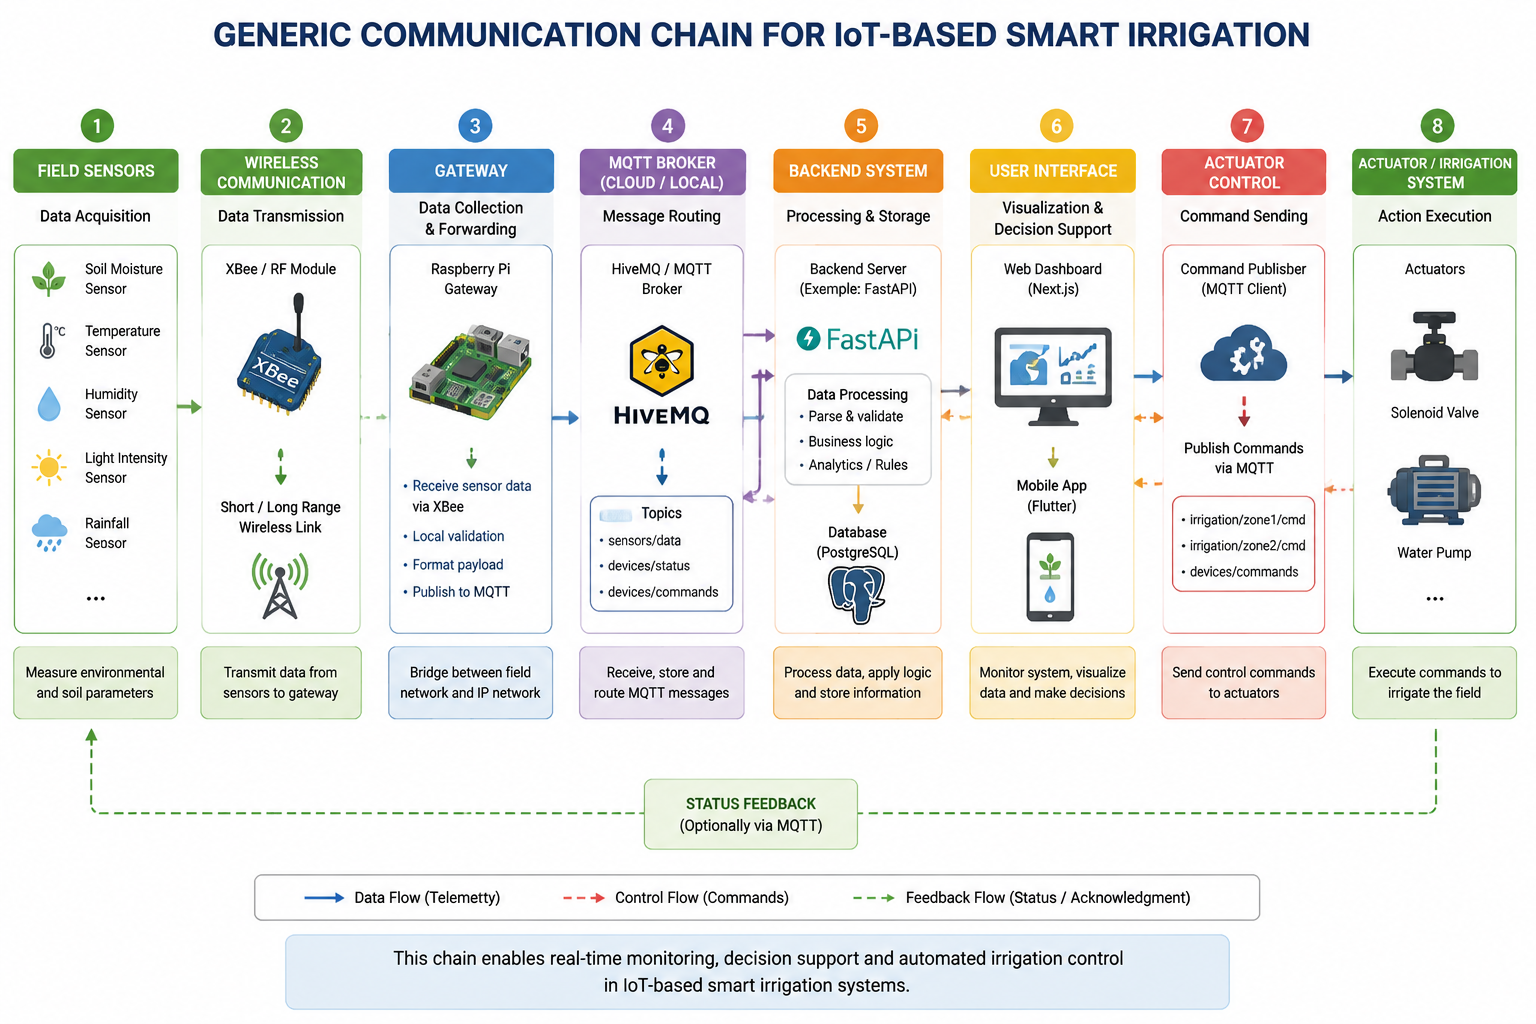
\includegraphics[width=0.9\textwidth]{figures/chapter_01/Figure 1.2 — Generic communication chain for IoT-based smart irrigation.png}
    \caption{Generic communication chain for IoT-based smart irrigation. Source: Authors.}
    \label{fig:1-2-generic-communication-chain-for-iot-based-smart-irrigation}
\end{figure}

\section{Actuators and irrigation control}

Actuators transform digital decisions into physical irrigation actions. In irrigation systems, common actuators include pumps, solenoid valves, relays, fertigation injectors, and motorized valves. In a smart irrigation architecture, actuation must be carefully controlled because an incorrect command can waste water or damage the prototype. Therefore, the system must distinguish between recommendation, validation, scheduling, and physical execution.

The Agrio prototype uses a WeMos device to control the pump through digital pins. In the current implementation, D5 is used for pump control and D3 is used for an auxiliary lamp. The backend publishes MQTT commands such as ON\_D5 and OFF\_D5 to the WeMos command topic. The WeMos publishes status messages indicating the state of D5 and D3. The dashboard reads the status through the backend and allows manual control or validated scheduled operation.

The system intentionally separates simulation from actuation. Running a Digital Twin simulation does not start the pump. Simulation only predicts a virtual outcome. Physical actuation occurs through explicit manual command or scheduled execution after validation. This design choice improves safety and makes the prototype more acceptable for academic demonstration.

\begin{figure}[H]
    \centering
    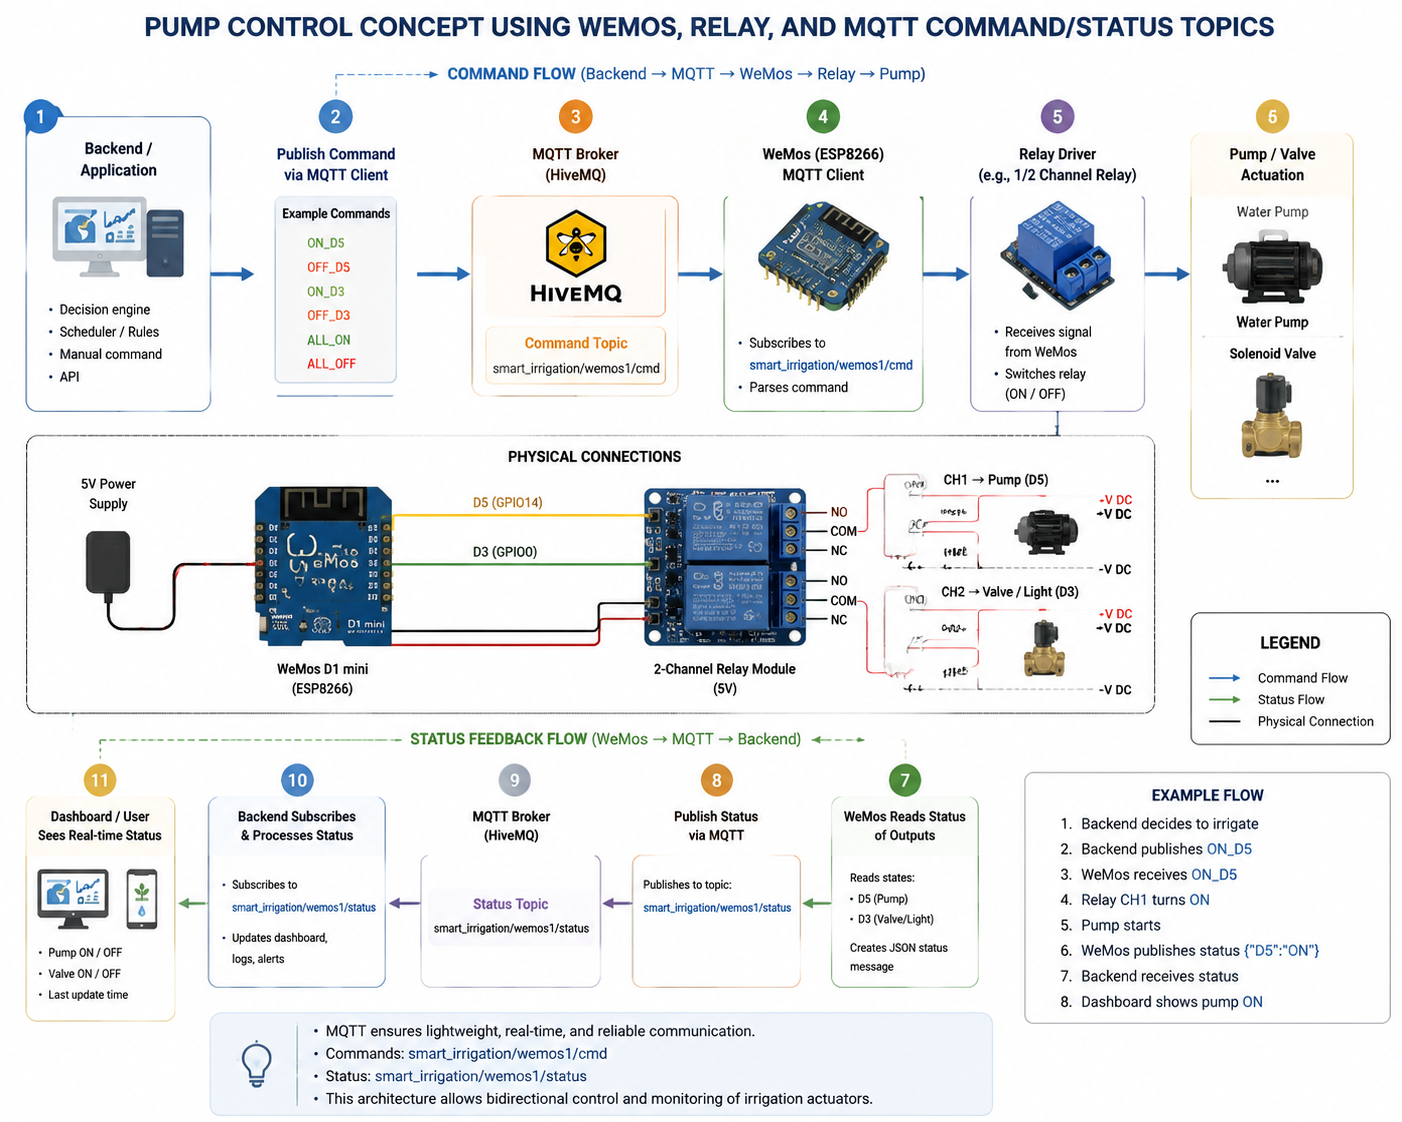
\includegraphics[width=0.9\textwidth]{figures/chapter_01/Figure 1.3 — Pump control concept using WeMos, relay, and MQTT commandstatus topics.png}
    \caption{Pump control concept using WeMos, relay, and MQTT command/status topics. Source: Authors.}
    \label{fig:1-3-pump-control-concept-using-wemos-relay-and-mqtt-command-status-top}
\end{figure}

\section{Challenges of smart irrigation systems}

The literature identifies several challenges that limit the adoption of smart irrigation: high sensor cost, sensor calibration, communication reliability, power management, data security, interoperability, model generalization, farmer acceptance, and limited long-term validation. The agricultural environment is also more variable than many industrial environments. Soil heterogeneity, crop growth, weather uncertainty, and biological responses make prediction and control difficult.

Many existing systems demonstrate promising results in laboratory or small-scale settings but lack extended field testing. This limitation is also relevant for Agrio. The current prototype demonstrates the complete technical workflow in a controlled environment, but long-term agronomic validation in real farm conditions remains future work. A rigorous academic thesis should therefore present both the strengths and limitations of the project transparently.

Another challenge is the gap between decision support and autonomous control. Fully automatic irrigation may be attractive, but it requires strong safety, calibration, and trust. Human-in-the-loop validation is a practical compromise for a final-year prototype: the system can recommend and simulate, while the user remains responsible for confirming or scheduling physical irrigation.

\section{Conclusion}

This chapter presented the context of precision agriculture and smart irrigation. It showed that irrigation optimization requires sensing, communication, data processing, decision support, and actuator control. The chapter also introduced the importance of soil moisture, weather variables, wireless communication, and safe pump control. These concepts prepare the transition toward Digital Twin technology, which is presented in the next chapter as the conceptual foundation of Agrio.
